%-------------------------------------------------------------------------
% INFORMACIÓN DEL ARTÍCULO
\thispagestyle{portadapage}
\setcounter{section}{0}
\setcounter{subsection}{0}
\setcounter{subsubsection}{0}
\setcounter{actividad}{0}
\setcounter{actividad_previa}{0}
\setcounter{actividad_entre}{0}
\renewcommand{\articulotipo}{Taller}
\renewcommand{\articulotitulo}{Descifrando los secretos de la pista: estadística y simulaciones en la Fórmula 1}
\phantomsection
\stepcounter{section}
\addcontentsline{toc}{section}{\protect\numberline{\thesection} \articulotitulo}
\desctotoc{del Valle Vides, C. N.; Chocobar, E. F.}

\begin{center}
	\setstretch{1.5}
	{\Huge \scshape
		\articulotitulo
	}
\end{center}

\noindent\rule{\linewidth}{2pt}

\vspace{0.25cm}

\begin{flushright}
	{\Large \scshape
		Cinthia Noelia del Valle Vides
	}\\
	{\large \itshape
		Universidad Nacional de Salta
	}\\
	{\ttfamily \small
		diamantecinthia@gmail.com
	}\\
	\vspace{1em}
	{\Large \scshape
		Ezequiel Francisco Chocobar 
	}\\
	{\large \itshape
		Universidad Nacional de Salta
	}
\end{flushright}

\vspace{0.5cm}

\begin{center}
	\begin{minipage}{0.75\linewidth} \small
		\textsc{Resumen}. ~
		Este taller consistirá, en líneas generales, en mostrar a los cursantes una aplicación tal vez poco conocida pero muy curiosa y utilizada de la Estadística descriptiva en el ámbito de la Fórmula 1, a través de una propuesta de trabajo con lotes de datos reales en la que se utilizarán los conceptos básicos de esta rama de la matemática, con ayuda del programa Microsoft Excel. A su vez, se espera que la propuesta pueda ser útil para aquellos asistentes que quizás se dedican a la enseñanza de la Estadística, de manera que a partir de ella sean capaces de pensar en otras propuestas didácticas originales para llevar a cabo con sus respectivos grupos de alumnos.
		
		Se trabajarán con los tiempos realizados por algunos de los pilotos en cada una de las vueltas de la Práctica 2 de un Gran Premio de F1, los cuales pueden ser organizados en una tabla. A partir de este lote de datos se pueden obtener resultados muy importantes para las escuderías como por ejemplo el promedio de vueltas, la vuelta rápida y/o lenta (valores alejados), el ritmo de carrera (qué tan consistente es el desempeño del binomio piloto-auto, es decir si este realiza vueltas muy rápidas pero también muy lentas o si logra mantener el ritmo en toda la carrera), estimar la degradación de los neumáticos, etc. y a su vez comparar los resultados del binomio analizado con los binomios contrincantes para predecir el resultado del Gran Premio.
	\end{minipage}
\end{center}
%-------------------------------------------------------------------------

\subsection{Introducción}

\subsubsection{Importancia del taller}

Este taller consistirá, en lineas generales, en mostrar a los cursantes una aplicación tal vez poco conocida pero muy curiosa y utilizada de la Estadística descriptiva en el ámbito de la Formula 1. A través de una propuesta de trabajo con lotes de datos reales en la que se utilizaran los conceptos básicos de esta rama de la matemática, con ayuda del programa Microsoft Excel. A su vez, se espera que la propuesta pueda ser útil para aquellos asistentes que quizás se dedican a la enseñanza de la Estadística, particularmente en el nivel medio y superior, de manera que a partir de ella sean capaces de pensar en otras propuestas didácticas originales para llevar a cabo con sus respectivos grupos de alumnos.

La Fórmula 1, abreviada como F1 y también denominada la «categoría reina del automovilismo», es la competición de automovilismo internacional más popular y prestigiosa, superando a otras categorías como la NASCAR, el Campeonato Mundial de Rally, el Campeonato Mundial de Turismo o la Fórmula E, entre otras. A cada carrera se le denomina Gran Premio y el torneo que las agrupa se denomina Campeonato Mundial de Fórmula 1. La entidad que la dirige es la Federación Internacional del Automóvil (FIA) y actualmente compiten en ella 10 escuderías con dos pilotos por cada una (que también compiten entre ellos), es decir un total de 20 pilotos. Pero es importante mencionar que, como explica \textcite{ramirez22}, un Gran Premio de Fórmula 1 no sólo es la carrera que se lleva a cabo los domingos, ni la sesión de calificación, aunque para los aficionados son los eventos más emocionantes. La actividad en pista comienza desde el viernes (en algunos casos extraordinarios, se adelantan al jueves) con las prácticas libres. En total, son tres sesiones de prácticas libres a lo largo del fin de semana de un Gran Premio, cada una de ellas con una duración de 60 minutos, las cuales resultan indispensables para los pilotos y los equipos.

La segunda sesión de entrenamientos es posiblemente la más importante (y es justamente la que nos interesa analizar en este taller), ya que se realiza a la misma hora (casi siempre) a la cual se desarrollará la carrera, por lo que los ingenieros obtienen información más precisa sobre el clima y la temperatura, lo cual es vital para conocer las condiciones y comportamiento de los neumáticos. De esta manera, los autos utilizan dos juegos de neumáticos, los mismos que se usarán en la carrera y en la calificación. Normalmente, los equipos usan los primeros 40 minutos para marcar tiempos rápidos, por lo que usan poco combustible (para hacer el auto más ligero) y eso arroja un panorama más claro de lo que podría suceder en la sesión de calificación. Los últimos 20 o 15 minutos, las escuderías optan por cargar el almacén de combustible hasta casi llenarlo. Esto hace que el auto sea más pesado y lento, y a esto se le conoce como “ritmo de carrera”, pues arroja datos y condiciones a lo que será el inicio de la carrera.

En este taller se trabajaran con los tiempos realizados por algunos de los pilotos en cada una de las vueltas de la \textit{Práctica 2}, los cuales pueden ser organizados en una tabla. A partir de este lote de datos se pueden obtener resultados muy importantes para las escuderías como por ejemplo el promedio de vueltas, la vuelta rápida, la vuelta lenta (valores alejados), el ritmo de carrera (que tan consistente es el desempeño del binomio piloto-auto, es decir si este realiza vueltas muy rápidas pero también muy lentas o si logra mantener el ritmo en toda la carrera), si hay tiempos de vuelta muy alejados a los demás, estimar la degradación de los neumáticos, etc. y a su vez comparar los resultados del binomio analizado con los binomios contrincantes para predecir el resultado del Gran Premio. Con estos resultados algunas veces las escuderías toman decisiones en cuanto estrategia o mecánica del automóvil para mejorar el rendimiento, pero el aporte mas importante de este estudio radica en lo que significa para la preparación mental del piloto y del resto del equipo para un posible resultado al final de la carrera, Efectivamente, todo esto no puede ser logrado sin la ayuda de la Estadística.

Para cursar este taller se necesita que los participantes tengan una computadora o tablet con Microsoft Excel descargado en versión 2016 o posteriores, o en su defecto alguna versión anterior y el software Geogebra. Esto se debe a que las versiones anteriores de Microsoft Excel no tienen la opción para realizar Diagramas de Cajas.

\subsubsection{Fundamentos}

De acuerdo a la definición que presenta \textcite{ahumada15}, «\textit{La estadística es la ciencia que estudia los métodos para recoger, organizar, resumir y analizar datos, así como para sacar conclusiones válidas para la toma de decisiones razonables en situaciones de incertidumbre}». De esta definición surgen dos ramas importantes de la estadística: Descriptiva e inferencial. La Estadística descriptiva tiene por objeto presentar y resumir los datos mediante cuadros, tablas y gráficos con la finalidad de describir las características del conjunto observado. Se obtienen conclusiones que no van más allá de ese conjunto. Las destrezas más importantes para la estadística son saber diseñar una observación, encuesta o experimento, utilizarla para obtener datos, analizarlos, presentarlos y a partir de ellos formular conclusiones. Es por esto que buscamos que en este taller los cursantes no solo sean capaces de realizar gráficos y utilizar formulas sino que puedan interpretar los resultados obtenidos en el contexto de la F1.

A continuación presentamos los principales conceptos matemáticos y/o estadísticos relevantes para la propuesta del taller:

De acuerdo a lo planteado por \textcite{ahumada15} es importante el modo en que se realiza el registro de datos con los que se va a trabajar. Uno puede, como en este caso, tomar registros o relevamientos ya realizados por otros. En la actualidad, el registro, o las mediciones son cada vez más precisas, con la ayuda de las nuevas tecnologías. Estos datos son valores observados de una \textbf{variable}, entendiendo como variable a la característica bajo estudio que puede tomar valores (o modalidades) diferentes. Esta variable podrá ser medida o no. En el caso de la propuesta de este taller la variable bajo estudio son los tiempos de vuelta realizados por cada binomio piloto-auto. Se trata de una variable cuantitativa continua dado que entre dos valores dados, la variable puede tomar cualquier valor intermedio (es importante destacar que las vueltas realizadas por los pilotos son superiores a un minuto e inferiores a 2 minutos, aquí que trabajaremos con tiempos considerando los segundos y hasta la décima de segundo). En la tabla de la figura \ref{fig:01} se muestra un ejemplo de un lote de datos presentado en forma de tabla, el cual consiste en los tiempos de vuelta realizados por un piloto determinado en un total de 12 vueltas de su Practica 2.


\begin{figure}[h!]
	\caption{Tiempos de vuelta.}
	\label{fig:01}
	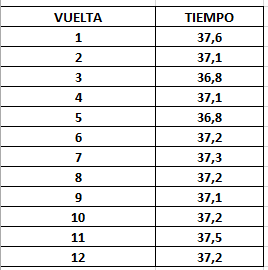
\includegraphics[width=0.3\linewidth]{Trabajos/01/Anexos/01.png}
\end{figure}

Los datos pueden organizarse de diferentes maneras. Para algunos tipos de datos, como los de esta propuesta por ejemplo, será conveniente la representación gráfica con una curva simple (\textbf{diagrama de líneas}). Es importante en este caso la escala elegida para los ejes, ya que la impresión visual del gráfico no debe ser exagerada en ningún sentido. Estos gráficos permiten visualizar de una sola vez la tendencia general y comparar simultáneamente varias tendencias. Esto se ve ejemplificado en la figura \ref{fig:02}, en donde en el eje horizontal aparecen el numero de vueltas que realizó el piloto y en el eje vertical el tiempo que le llevo realizar dicha vuelta. Como se dijo anteriormente, en el ejemplo consideramos valores como $36.8$ segundos, que en realidad indican que un piloto hizo una vuelta de 1 minuto con $36,8$ segundos.

\begin{figure}[h!]
	\caption{Gráfico de líneas.}
	\label{fig:02}
	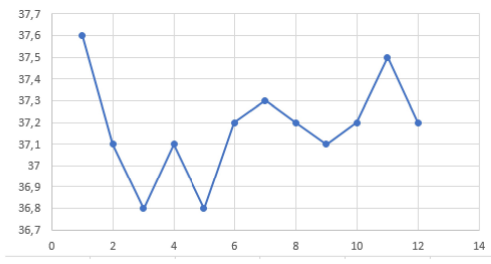
\includegraphics[width=0.6\linewidth]{Trabajos/01/Anexos/02.png}
\end{figure}

Cuando tenemos variables continuas, organizamos la tabla de frecuencias definiendo intervalos de clase. Esta tabla permite realizar un gráfico llamado \textbf{histograma}. Para realizar dicho histograma los datos se clasifican en intervalos y en cada uno de ellos se representa la frecuencia correspondiente con una barra. Los datos se agrupan con el fin de brindar información más rápida, pero al formar los intervalos se pierde la información puntual, por lo tanto se debe cuidar no perder demasiada información. En el histograma, las frecuencias de clase están representadas por el área de la barra en cada clase. Por esto la altura de cada barra, será la frecuencia dividida por la amplitud del intervalo. Si los intervalos son de la misma amplitud, se puede realizar el histograma usando las frecuencias como alturas, ya que en ese caso el diagrama es el mismo, sólo sufre un cambio de escala que no modifica la información mostrada.

Dentro de lo posible, es conveniente trabajar con intervalos de igual amplitud. Sobre el histograma se dibuja el \textbf{polígono de frecuencias} que se obtiene uniendo los puntos medios de la parte superior de cada barra; se suele agregar intervalos de frecuencia cero al comienzo y al final, para comenzar y terminar el polígono en el eje. El polígono de frecuencias muestra la misma información que el histograma, pero da una idea de crecimiento o decrecimiento más real que las barras del histograma.

En la figura \ref{fig:03} se muestra un ejemplo de un histograma realizado a partir de los tiempos obtenidos por un piloto en una simulación de carrera como las que se estudiaran en el taller (los mismos de la tabla de la figura \ref{fig:01} y a partir de los que se realizo el grafico de lineas de la figura \ref{fig:02}). Sobre el eje horizontal aparecen las marcas de clase, es decir el punto medio del intervalo.

\begin{figure}[h!]
	\caption{Ejemplo de un histograma construido a partir de los tiempos realizados.}
	\label{fig:03}
	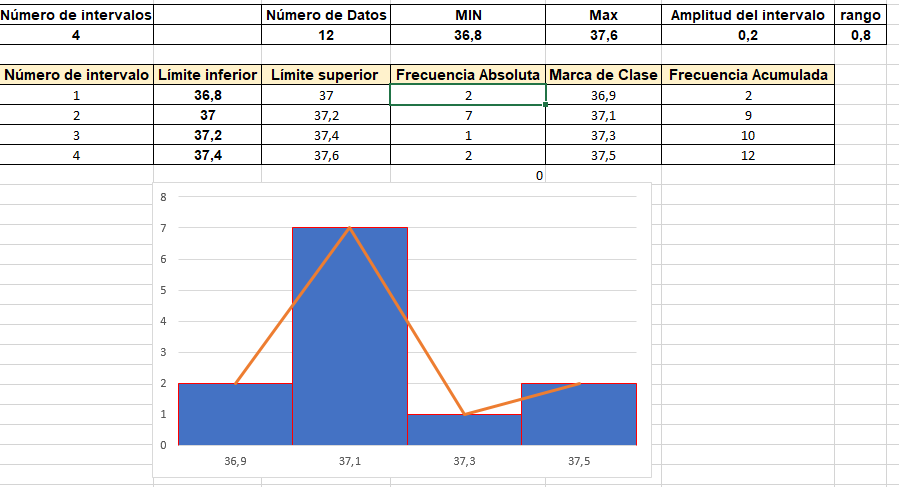
\includegraphics[width=0.8\linewidth]{Trabajos/01/Anexos/03}
\end{figure}

A partir de un lote de datos, \textcite{walpole12} menciona las siguientes medidas de localización o posición:
\begin{itemize}
	\item \textbf{Media aritmética}: Supongamos que las observaciones en una muestra son $x_{1}, x_{2}, \dots ,x_{n}$. La media de la muestra se denota con $\overline{x}$ y es $\overline{x} = \sum_{i=1}^{n} \frac{x_{i}}{n} = \frac{x_{1} + x_{2} + \dots + x_{n}}{n}$
	
	\item \textbf{Mediana}: Supongamos que las observaciones en una muestra son $x_{1}, x_{2}, \dots, x_{n}$ ordenadas de forma creciente. La mediana de la muestra dependerá de si $n$ es par o impar: $$\widetilde{x} = \begin{cases}
		x_{\frac{n+1}{2}} & \text{impar}\\
		x_{\frac{n}{2}} & \text{par}
	\end{cases}$$
\end{itemize}

\textcite{ahumada15} menciona otras medidas de posición que son importantes para los casos analizados en este taller que son los \textbf{cuartiles}:
\begin{itemize}
	\item \textbf{Primer cuartil}: Se denomina primer cuartil ($Q_{1}$) al número real tal que a lo sumo el 25\% de los datos son menores que él y a lo sumo el 75\% son mayores.
	\item \textbf{Segundo cuartil}: Coincide con la mediana $\widetilde{x}$.
	\item \textbf{Tercer cuartil}: Se denomina primer cuartil ($Q_{3}$) al número real tal que a lo sumo el 75\% de los datos son mayores que él y a lo sumo el 25\% son mayores.
\end{itemize}

\noindent También son importantes las medidas de dispersión:
\begin{itemize}
	\item \textbf{Rango}: Es la diferencia entre el menor y el mayor valor de la variable.
	
	\item \textbf{Rango intercuartil}: Es la diferencia entre el primer cuartil y el tercer cuartil. 
	
	\item \textbf{Varianza:} Se define como el promedio de los cuadrados de las desviaciones respecto de la media. $$\sigma^{2} = \frac{\sum_{i=1}^{n} (x_{i} - \overline{x})^{2}}{n}$$
	
	\item \textbf{Desviación estándar}: Se define como la raíz cuadrada de la varianza. Mide la dispersión de los datos, es decir, mientras más dispersos se encuentren los datos mayor es su desviación estándar. 
\end{itemize}

Ahora bien, describir un lote de datos significa hacer referencia, entre otras cosas, a la posición, dispersión, forma, que tal lote presenta para realizar un análisis y sacar conclusiones acerca del mismo. La técnica que utilizaremos para el análisis exploratorio de datos en este caso es el \textbf{Diagrama de Cajas} o comúnmente conocido como \textbf{\textit{box plot}}. 

Este diagrama consiste en una caja a lo largo del eje de la variable, donde se encuentra el 50\% central de los datos (o sea que incluye los dos cuartos centrales), y el resto constituyen las colas de la distribución (el primer cuarto, la cola izquierda; el cuarto, la cola derecha), representadas por segmentos a los costados de la caja. Si hay valores muy extremos, las colas no comienzan en los extremos sino que se destacan estos valores con una marca y la cola comienza en el dato inmediato siguiente. En la figura \ref{fig:04} se muestra un ejemplo de un \textit{box plot} que muestra la información del lote datos presentado en la tabla de la figura \ref{fig:02}.

\begin{figure}[h!]
	\caption{Box Plot - Max Verstappen}
	\label{fig:04}
	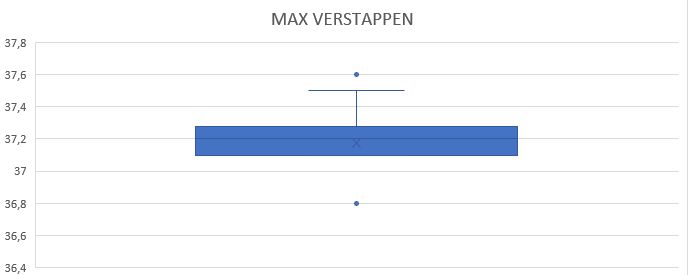
\includegraphics[width=0.6\linewidth]{Trabajos/01/Anexos/04}
\end{figure}

Como vemos, la simplicidad del dibujo hace que notemos rápidamente  en él las características importantes, como por ejemplo:
\begin{itemize}
	\item \textbf{Valores alejados}: se distinguen por las marcas especiales que lo separan del resto del diagrama. 
	\item \textbf{Posición}: el eje de la variable dará los valores de las medidas, especialmente se observa la posición de la mediana aunque también se puede agregar la posición de la media.
	\item \textbf{Dispersión}: cajas anchas nos sugieren distribuciones muy dispersas en la parte central mientras que cajas angostas nos muestran una gran concentración de datos (teniendo en cuenta que el ancho de la caja es el rango intercuartil). La longitud de las colas por su parte nos dirá la mayor o menor concentración de los datos en las zonas extremas. 
\end{itemize}

De esta manera, como se menciono anteriormente, estos conceptos nos permitirá no solo conocer el desempeño de los binomios piloto-auto durante las practicas sino también realizar algunas predicciones sobre la carrera entendiendo el “predecir” como razonar sobre el futuro
con base en una experiencia previa.

Por otra parte, como mencionamos en la introducción, uno de los objetivos principales de este taller es mostrar una aplicación curiosa de la Estadística en la Formula 1. Motiva nuestro interés en parte los aportes de \textcite{migueldeguzman02} en los que menciona la importancia de que el aprendizaje de las matemáticas no se realice explorando las construcciones matemáticas en si mismas sino en continuo contacto con las situaciones del mundo real que les dieron y dan motivación y vitalidad. El autor resalta el gran poder motivador que la modelización y las aplicaciones poseen y es justamente por esto que creemos que la propuesta permitirá desarrollar un interés por las aplicaciones de la Estadística (particularmente en el mundo deportivo) permitiendo así la creación de un espacio de aprendizaje ameno. 

De acuerdo a \textcite{bressan08} las graficas o gráficos tienen la enorme ventaja de permitir apreciar con una rápida mirada una notable cantidad de información; por ello la propuesta le pide a los cursantes la realización de diferentes gráficos para destacar las características y la información que brinda cada uno de ellos. Por otro lado, los autores destacan que uno de los objetivos fundamentales de la estadística es poder dar un conjunto reducido de valores que puedan resumir en forma adecuada una gran cantidad de información; en nuestro caso particular buscaremos resumir los resultados mas importantes de la Practica 2 a través de las medidas de dispersión y posición mas importantes y de los gráficos que pueden realizarse. Mencionan ademas algunos ordenes de dificultad en la aprehensión del concepto de media aritmética o promedio entre los cuales nos interesan los siguientes:
\begin{itemize}
	\item El promedio puede eventualmente ser diferente a todos los valores observados. Buscamos hacer hincapié en que lo que se calcula es un promedio de vueltas obtenido por un piloto que podría no coincidir con ningún tiempo de vuelta realizado por dicho piloto.
	\item Si bien el promedio es una cantidad muy importante, un lote de datos tiene mucha información y características que el promedio no expresa. Veremos como tal vez un piloto puede tener un mejor promedio de vueltas que otro y sin embargo terminar por detrás de este a causa de otras características importantes como por ejemplo el ritmo de carrera.
\end{itemize}

Con respecto al trabajo con Excel, \textcite{valverde10}, en un articulo que habla entre otras cosas sobre la importancia de que el docente tenga incorporados no solo el conocimiento disciplinar y pedagógico sobre lo que desea enseñar sino que también es importante el conocimiento de la tecnología que puede utilizar en dicha enseñanza, nos mencionan que el software es un producto nunca acabado, siempre por pulir, susceptible de ser alterado para cumplir nuevas funciones y que para algunos profesores esto es difícilmente asumible y admisible dentro de un aula. El hecho de que la mayoría del software esté diseñado para contextos no educativos contribuye aún más a esta opacidad. De esta manera, adaptar software de propósito general del entorno laboral (por ej. las hojas de cálculo) a la práctica escolar requiere trabajar a través de la opacidad para reconfigurar y modificar sus propósitos iniciales a las necesidades educativas. Teniendo en cuenta esto y la necesidad de la preparación de los profesores en los usos educativos de la tecnología para el desarrollo de Buenas Prácticas educativas con TIC es que se ha pensando en una propuesta que permita visualizar lo útil que resulta el uso del software Excel y/o GeoGebra a la hora de trabajar con Estadística y la importancia de su inclusión en las propuestas didácticas. Los autores mencionan además que aunque las administraciones educativas han dedicado en los últimos años un importante esfuerzo en la formación tecnológica del profesorado en actividad, y sobre todo durante y después de la pandemia, lo cierto es que en la actualidad aún son muchos los profesores que no se consideran competentes para abordar la integración de las TIC en sus prácticas docentes y que, en consecuencia, no han descubierto la relevancia de estos nuevos medios para el aprendizaje. Entonces esperamos que este espacio aporte a esta cuestión, creando también un espacio de trabajo colaborativo con herramientas digitales. 

Con respecto a la evaluación \textcite{crippa98} menciona la importancia en que no solo se evalúen contenidos sino también habilidades actitudes y procedimientos. Por otro lado también menciona las “evaluaciones sin prueba” ya que una de sus ventajas es que permite evaluar también los aspectos mencionados anteriormente. Uno de los ejemplos de este tipo de evaluaciones es justamente lo que la autora denomina como “Evaluación por medio de carpetas o \textit{portfolios}” y que consiste en que los alumnos confeccionen una carpeta que incluya algunas de sus producciones en base a criterios propuestos por el docente. Esto propicia entonces por ejemplo fomentar la exposición de los propios procedimientos, valorar la planificación, estructuración y adaptación continua a una situación problemática, establecer relaciones interdisciplinarias a través del trabajo con problemas relativos a otros contextos. Es por esto que a la hora de pensar la evaluación final y teniendo en cuenta que el publico destinatario del taller serán estudiantes de profesorados y docentes se propone la elaboración grupal de un documento que hará de alguna manera el papel de carpeta en donde presentará un resumen de los trabajado en el taller. Aquí se evaluara también la capacidad de trabajar en equipo, la presentación en tiempo y forma de lo pedido, la habilidad para el uso de software como Excel, la explicitación de los procedimientos matemáticos que se utilizan para llegar aun cierto resultado, etc.

\subsection{Contenidos}

Los contenidos que se desarrollaran a lo largo del taller son:
\begin{itemize}
	\item Variables cuantitativas continuas.
	\item Grafico de lineas
	\item Histogramas
	\item Diagramas de caja - box plot
	\item Medidas de posición: Media aritmética, mediana y cuartiles 
	\item Medidas de dispersión: Rango, Rango intercuartil, Desvío.
	\item Funciones de Excel para calculo de medidas y realización de gráficos estadísticos.
\end{itemize}

\subsection{Requisitos previos}

\begin{itemize}
	\item Conocer nociones muy básicas de Excel (como por ej: tipeado de datos en una tabla y ordenamiento de los mismos)
	\item Tener descargado Excel en su versión 2016 en adelante o bien una versión previa conjuntamente con el programa GeoGebra.
	\item Haber realizado algún curso previo sobre nociones básicas de estadística descriptiva (Manejar conceptos de medidas de posición y dispersión de un lote de datos y armado de gráficos de linea e histogramas).
\end{itemize}

\subsection{Objetivos}

Que el asistente al taller sea capaz de: 
\begin{itemize}
	\item Utilizar Excel para realizar un histograma a partir de una muestra de tiempos de vueltas realizadas por pilotos de F1 en una simulación de carrera.
	\item Obtener, con ayuda del programa, las medidas de posición y dispersión del lote de datos.
	\item Construir un boxplot que modelice la situación presentada en las simulaciones. 
	\item Interpretar el boxplot teniendo en cuenta las medidas de dispersión y posición y sacar conclusiones sobre el rendimiento del binomio auto-piloto a partir de él.
	\item Realizar predicciones para la carrera a partir de los datos obtenidos comparando su trabajo con el de sus compañeros. 
\end{itemize}

\subsection{Actividades}

\subsubsection{Actividades previas}

En el periodo de actividades previas los cursantes tendrán acceso a una presentación en la que se encontrará un breve resumen de los conceptos teóricos de Estadística que serán de gran utilidad para el inicio del taller. Específicamente, estamos hablando de los conceptos de variables cuantitativas continuas, gráficos de lineas medidas de posición y dispersión mas importantes y armado de histogramas, a modo de repaso. Seguidamente, los cursantes deberán desarrollar la siguiente actividad. 

\begin{actividad_previa}
	En la siguiente lista se muestran los campeones del Mundial de Formula 1 y al lado la edad con la que salieron campeón por primera vez (en algunos casos es la única):
	
	\begin{figure}[h!]
		\caption{Tabla de Edades de pilotos Campeones del mundo}
		\label{fig:05}
		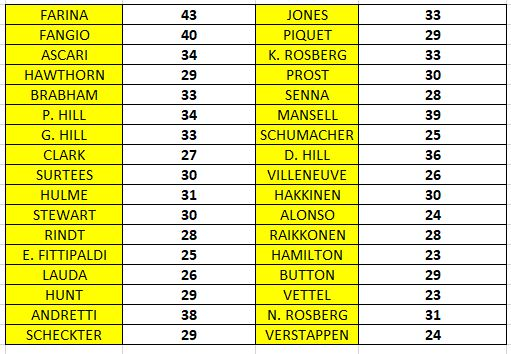
\includegraphics[width=0.6\linewidth]{Trabajos/01/Anexos/05}
	\end{figure}
	
	\begin{enumerate}[a)]
		\item Analizar los siguientes datos obteniendo así las medidas de posición del lote:
		
		\begin{enumerate}
			\item Edad promedio con la que salieron campeones estos pilotos. 
			
			\item Edad del piloto más longevo y más joven en acceder al titulo.
			
			\item Cuartiles 1, 2 y 3 del lote de datos y el rango intercuartil.
			
			\item Desvío estándar. ¿Qué crees que representa este valor?
		\end{enumerate}
		
		\item A partir de estos resultados desarrollar los siguientes incisos:
		
		\begin{enumerate}
			\item Realizar un gráfico de lineas colocando en el eje horizontal los nombres de los pilotos, y en el eje vertical la edad correspondiente.
			
			\item Realizar un histograma teniendo en cuenta el lote de datos presentado, determinando los intervalos que te resulten mas convenientes.
			
			\item ¿Qué características del lote de datos se aprecian mejor en cada uno de los gráficos realizados anteriormente?
			
			\item Escribir una conclusión que resuma todo lo trabajado con la información brindada sobre las edades de los pilotos.
		\end{enumerate}
	\end{enumerate}
\end{actividad_previa}

El objetivo de esta propuesta es introducir a los asistentes al trabajo relacionado con la obtención de medidas de posición y dispersión, realización de gráficos estadísticos y elaboración de conclusiones a partir de un cierto lote de datos. 

Además los cursantes tendrán acceso a un glosario online con los términos mas usados en la Formula 1 para que puedan ir familiarizándose con ellos. El mismo será similar al que se encuentra en el siguiente enlace \url{https://holatelcel.com/holatelcel/glosario-basico-para-entender-la-formula-1/}.

\subsubsection{Primera hora y media presenciales}

Este encuentro se realizará teniendo en cuenta la siguiente organización con tiempos estimativos sujetos a las diferentes eventualidades que pudieren surgir:

\begin{enumerate}
	\item Breve presentación de las personas a cargo del taller, breve sondeo sobre las trayectorias previas de los cursantes haciendo hincapié en sus experiencias con la Estadística y explicación de los requisitos para la aprobación del taller (15 min.).
	
	\item Explicación de que es lo que se busca estudiar y analizar principalmente en este taller, como así también de lo que se necesita manejar para realizar dicho trabajo. (10 min.).
	
	\item Explicación de los conceptos mas importantes de la Fórmula 1 que se necesitan conocer en este taller con participación activa de los asistentes, teniendo en cuenta el glosario que tenían para leer en la etapa de actividades previas y haciendo hincapié en nuestro objeto de estudio. (20 min.).
	
	\item Revisión de la tarea realizada sobre la edad de los pilotos, haciendo un repaso de los conceptos estadísticos que tenían para leer. (25 min.).
	
	\item Orientaciones para las actividades entre clases, enfatizando en el uso de Excel para la obtención de medidas de posición y dispersión y gráficos estadísticos (20 min.).
\end{enumerate}

\textbf{Observación}: Se utilizará como soporte una presentación de Power Point o herramientas similares que estará al alcance los alumnos en la plataforma Moodle después de la clase.

\subsubsection{Primeras dos horas entre clases}

En este tiempo los cursantes deberán desarrollar la siguiente consigna:

\begin{actividad_entre}
	Teniendo en cuenta el lote de datos de la actividad previa ahora obtener las medidas de posición y dispersión solicitadas y realizar los gráficos pedidos utilizando el software Microsoft Excel, teniendo en cuenta lo visto en clase.
\end{actividad_entre}

El objetivo de esta tarea es que los cursantes se familiaricen con el uso de Excel en el ámbito educativo y de la Estadística.

\subsubsection{Segunda dos horas presenciales}

Este encuentro se realizará teniendo en cuenta la siguiente organización con tiempos estimativos sujetos a las diferentes eventualidades que pudieren surgir:

\begin{enumerate}
	\item Revisión de tarea, espacio para dudas y consultas sobre lo realizado hasta ahora. (15 min.).
	
	\item Explicación de un ejemplo de simulación de carrera con los tiempos realizados por uno de los pilotos (en este caso el ultimo campeón del mundo Max Verstappen que son los que se muestran en la figura \ref{fig:01}). Los encargados del taller mostraremos como obtener, utilizando Excel, un grafico de lineas que represente la situación (como el que se presenta en la figura \ref{fig:02}), las principales medidas de posición y dispersión, un histograma a partir del lote de datos presentado (como lo que se muestra en la figura \ref{fig:03}) y las conclusiones que se pueden sacar sobre el desempeño de ese binomio piloto-auto a partir de lo trabajado. (30 min.).
	
	\item Los cursantes deberán formar equipos de 2 o 3 integrantes para realizar la siguiente actividad. A cada equipo se le asignara una tabla Excel con los tiempos realizados por un piloto distinto durante una simulación de carrera (30 min.).
	
	\begin{actividad}
		~
		\begin{enumerate}[i.]
			\item Con los datos facilitados en la Tabla Excel realizar un gráfico de lineas que contemple el N° de vuelta y el tiempo de la misma. 
			\item Dada la simulación de carrera, utilizar los comandos necesarios para determinar:
			\begin{enumerate}[a.]
				\item Vuelta más rápida de la simulación.
				\item Vuelta más lenta de la simulación.
				\item Tiempo medio de vuelta por compuesto de neumático.
				\item Entre qué tiempos estuvo la mayor consistencia de vueltas.
				\item Cuál fue el rango de tiempos teniendo en cuenta el promedio.
				\item Desviación estándar correspondiente al lote de datos. ¿Qué representa este valor?
			\end{enumerate}
			\item Realiza una tabla de frecuencias teniendo en cuenta el número de intervalos que considere conveniente y los datos de la simulación, y a partir de ella construye un histograma con su correspondiente polígono de frecuencias. 
		\end{enumerate}
	\end{actividad}
	
	\item Explicación de en que consiste un boxplot y como realizar uno utilizando Excel, con el ejemplo de simulación de carrera de Max Verstapen. Análisis del Box Plot obtenido (como el de la figura \ref{fig:04}) para determinar el desempeño del binomio piloto-auto durante la simulación, especialmente haciendo énfasis en el ritmo de carrera y la consistencia de vueltas. (30 min.). 
	
	\item Orientaciones para el desarrollo de la actividad entre clases (15 min.). 
\end{enumerate}

\textbf{Observacion}: En el caso de que haya cursantes que no cuenten con una versión de Excel del 2016 en adelante, se explicara como realizar el box plot utilizando el software GeoGebra. Esto se debe a que las versiones anteriores no permiten realizar Diagramas de cajas de manera sencilla como si se puede en las versiones mas actuales.

\subsubsection{Segundas dos horas entre clase}

Los cursantes deberán realizar la siguiente actividad con los mismos grupos que realizaron la actividad de clase.

\begin{actividad_entre}
	~
	\begin{enumerate}
		\item A partir de los datos obtenidos en la actividad anterior (de clase) y teniendo en cuenta las medidas de posición y dispersión realizar un diagrama de cajas y bigotes en Microsoft Excel.
		
		\noindent 2. Analizar los datos obtenidos a partir del boxplot y escribir una conclusión relacionando los mismos con el desempeño del binomio piloto-auto asignado.
		
		\noindent 3. Compara el box plot obtenido con el grafico de lineas y el histograma realizado previamente. ¿Qué características importantes de la simulación pueden apreciarse mejor en cada uno de ellos?. ¿Cuál permite visualizar mejor el ritmo de carrera y la consistencia de vueltas?
	\end{enumerate}
\end{actividad_entre}

\textbf{Observación}: Tanto al final de la segunda clase presencial como en el espacio asignado para la segunda actividad entre clases de la plataforma Moodle se les comunicará a los cursantes que al inicio de la tercera clase presencial deberán exponer por grupos sus desarrollos y conclusiones de lo trabajado en la actividad de la segunda clase y la segunda actividad entre clases (se proyectarán los archivos Excel de cada grupo para que puedan realizar sus exposiciones).

\subsubsection{Terceras dos horas presenciales}

\noindent Este encuentro se realizará teniendo en cuenta la siguiente organización con tiempos estimativos sujetos a las diferentes eventualidades que pudieren surgir:

\begin{enumerate}
	\item Revisión de la ultima tarea asignada (15 min.).
	
	\item Exposición de lo trabajado en grupos en la actividad de la segunda clase presencial y la segunda actividad entre clases (45 min.).
	
	\item Análisis general de los ejemplos de simulación propuestos y realización de una comparación entre ellos para realizar predicciones sobre la carrera. Se presentaran en pantalla todos los diagramas de caja , incluido el de Max Verstapen para comparar el desempeño de cada uno de los binomios piloto-auto durante la Practica 2 (por medio de una imagen similar a la de la figura \ref{fig:06} ) y en base a dicho análisis realizar predicciones sobre los resultados de la carrera (quien ganara, quien quedara en el podio, etc) con participación activa de los cursantes. (30 min.).
	
	\item Comparación de los resultados obtenidos durante la simulación con los tiempos realizados en la carrera por los pilotos, para ver cuanto coinciden las predicciones realizadas con los resultados del Gran Premio. Reflexión sobre la forma de los box plot realizados con los tiempos de la P2 y los realizados con los tiempos de la carrera (que se mostraran en pantalla para dicha comparación). (10 min.).
	
	\item Explicación de la evaluación final del taller (10 min.). 
	
	\item Breve charla sobre la experiencia de los cursantes en el taller y si las expectativas fueron cumplidas (10 min.).
\end{enumerate}

\begin{figure}[h!]
	\caption{Box Plot de varios pilotos}
	\label{fig:06}
	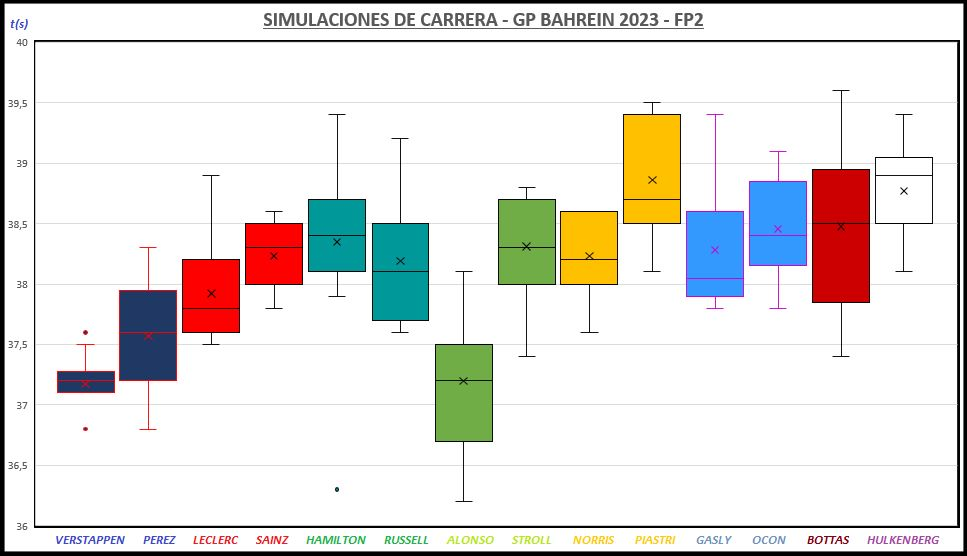
\includegraphics[width=0.8\linewidth]{Trabajos/01/Anexos/06}
\end{figure}

\subsubsection{Evaluación final}

Los cursantes tendrán un plazo de 1 semana para entregar la evaluación final grupal (con los mismos grupos de trabajo armados anteriormente) cuyas consignas son las siguientes: 

\begin{enumerate}
	\item Organizar en un documento (Word, LaTeX, etc) todo lo desarrollado en el taller a partir de la simulación de carrera del piloto asignado y una conclusión final que contenga el análisis y comparación general de todos los box plot realizados por los diferentes grupos (teniendo en cuenta lo debatido en la ultima clase y las predicciones realizadas).
	
	\item Escribir una reflexión sobre la posible inclusión de una propuesta didáctica similar en alguno de los niveles educativos (secundario, terciario o universitario a elección del grupo) justificando sus opiniones y, en caso de que corresponda, describir de manera general que cambios le realizarían para dicha inclusión. 
\end{enumerate}

\noindent Se calificará dicha evaluación con una escala numérica del 1 al 100 y se tendrán en cuenta los siguientes criterios de evaluación:
\begin{itemize}
	\item Presentación en tiempo y forma (20 p.).
	\item Utilización de Procedimientos matemáticos validos y acordes a lo requerido por las consignas presentadas (20 p.).
	\item Utilización del vocabulario propio de la estadística y de la Formula 1 (10 p.).
	\item Manejo del software Excel para la obtención de medidas estadísticas y realización de gráficos (10 p.).
	\item Organización adecuada del texto con el uso de gráficos e imágenes pertinentes. (10 p.).
	\item Interpretación de los resultados obtenidos en el contexto de la F1 (15 p.).
	\item Reflexión final clara y con su debida justificación (correspondiente al inciso 2 de la evaluación) (15 p.).
\end{itemize}

\subsection{Bibliografía}

\nocite{*}
\printbibliography[keyword={01}]